\documentclass[12pt]{article}

\usepackage[table]{xcolor}
\usepackage{amsmath}
\usepackage{graphicx}
\usepackage{setspace}
\usepackage{parskip}
\usepackage[top=1in,bottom=1in,left=1in,right=1in]{geometry}
\usepackage{booktabs}
\usepackage{dcolumn} %for use with R package stargazer
\usepackage{multirow}
\usepackage{rotating}

\interfootnotelinepenalty=10000

\usepackage{natbib}
\usepackage{hyperref}
\usepackage[hang,flushmargin]{footmisc} 
\hypersetup{pdfstartpage=1,
            pdfpagemode=UseNone,
            pdfstartview=FitH,
            pdffitwindow=true,
            colorlinks=true,
            linkcolor=blue,
            citecolor=blue}

\title{Contingent work in the United States: Less likely, but more concentrated}
\author{Jonathan P. Latner\thanks{Corresponding author: Jonathan Latner (\url{jonathan.latner@uni-bamberg.de}).  Universit{\"a}t Bamberg.  This project has received funding from the European Research Council (ERC) under the Horizon 2020 research and innovation program (grant agreement No 758491)}}

\date{\vspace{-5ex}}

\usepackage{pdflscape} % for 'landscape' environment
\usepackage{longtable}
\usepackage{lscape}

% define lightgray
\definecolor{lightgray}{gray}{0.9}

% alternate rowcolors for all long-tables
\let\oldlongtable\longtable
\let\endoldlongtable\endlongtable
\renewenvironment{longtable}{\rowcolors{5}{white}{lightgray}\oldlongtable} {
\endoldlongtable}

\begin{document}

\maketitle

{\bf Revision date:} \today

\section{Introduction}

These figures show preliminary analysis of trends in the United States on contingent work.  There are two sources of data.  The first is cross-sectional data from the Current Population Survey (CPS), Contingent Worker Supplement (CWS).  The CWS is a cross-sectional survey.  It was conducted in 1995, 1997, 1999, 2001, 2005, and 2017.  Sample are prime-aged workers (25-54).  Contingent work is the `broadest' measure, defined as wage and salary workers who believe their job will not last.  The CWS also includes variables on alternative employment arrangements, including includes contract worker, temp help agency, and on-call/day laborer.  Independent contractor is a separate category, primarily self-employed individuals.  

The second source of data is from the Census, Survey of Income and Program participation (SIPP).  The SIPP is a panel survey, conducted every 4 months, i.e. 3 waves per year.  While most panel periods are 4 years long, the 2001 panel is 3 years long and the 2008 panel was 5 years long.  We limit each sample to 3 years or 9 waves.  Sample are prime age (25-54) and must be employed or unemployed in each wave of a given panel.  Contingent work is defined by two types of respondents.  First, those who state that they do not have a definite arrangement to work on an ongoing basis, they have some `other' work arrangement—defined as including odd jobs, on-call work, day labor, one-time jobs, and informal arrangements \citep{gao_2015}.  Second, those who are employed in the personnel supply services (SIC 736) or employment services industry (SIC 5613), depending on the year, which includes those working for temporary help agencies and employment agencies \citep{lane_etal_2003}.

The results confirm previous research based on the CWS (cross-sectional data), see figure \ref{graph_cps_rate}.  Contingent work is not rising over time in the United States.  

The contribution is the use of the SIPP (panel data), to examine contingent work over time within individuals.  When we use the SIPP in its cross-sectional form to examine the rate of contingent work, we replicate the stagnating levels found in the CWS (figure \ref{graph_sipp_rate}).  However, when we use the SIPP as a panel, we can see that the risk of experiencing at least 1 wave (out of 9) with contingent work in a 3-year panel period is {\emph declining}, as shown in figure \ref{graph_sipp_risk}.  At the same time, conditional on the experiencing at least 1 wave of contingent work, the average number of waves with contingent work is rising (figure \ref{graph_sipp_number_avg}).  The interpretation is that even if the risk of contingent work is declining, contingent work is becoming more concentrated among already individuals whose employment is already precarious.

% Some suggest that this finding is biased because the CWS only asks about an individuals primary source of employment, which underestimates levels and trends in contingent work \citep{howell_kalleberg_2019}.  However, even studies that do account for secondary or tertiary forms of labor do not necessarily find increasing levels of contingent work \citep{katz_etal_2019}, or, if they do, it is related to independent contract work, which may or may not be contingent.


%%%%%%%%%%%%%%%%%%%%%%%%%%%%%%%%
% Graphs
%%%%%%%%%%%%%%%%%%%%%%%%%%%%%%%%
\section{Figures}

\begin{figure}[htp!]
    \caption{Trends in levels of contingent work over time (CWS)}
    \resizebox{\textwidth}{!}{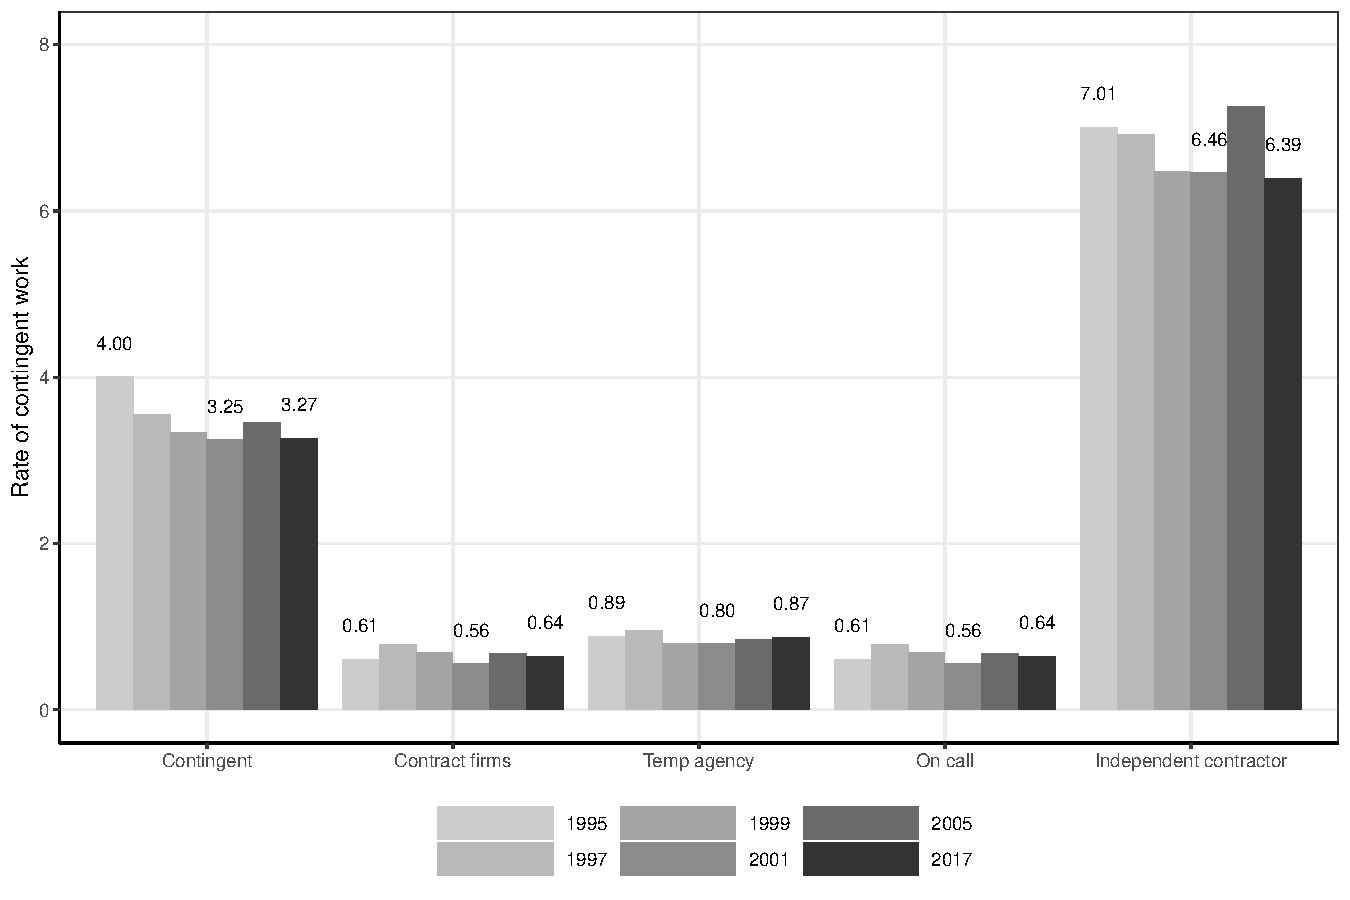
\includegraphics{../graphs/graph_cps_rate.pdf}}
    \label{graph_cps_rate}
    \footnotesize{Note: The interpretation of the figure is that, the share of workers who are contingent has fallen over time.  Authors calculations using data from CWS.  Figure replicates \citep[Fig. 5]{howell_kalleberg_2019} and  \cite[Fig 4-2]{abraham_houseman_2022}.}
\end{figure}

\begin{figure}[htp!]
    \caption{Trends in levels of contingent work over time (SIPP)}
    \resizebox{\textwidth}{!}{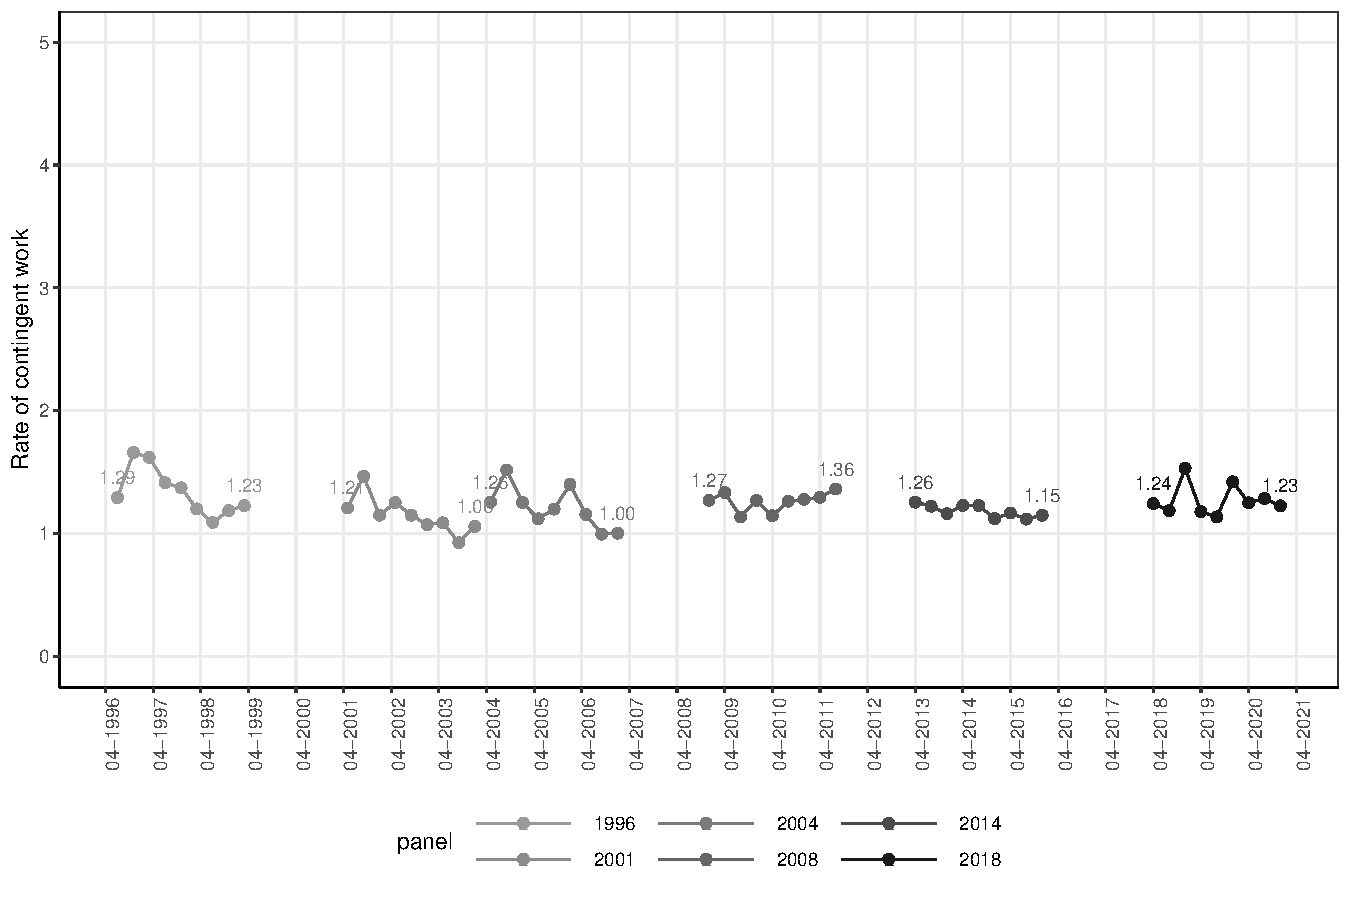
\includegraphics{../graphs/graph_sipp_rate.pdf}}
    \label{graph_sipp_rate}
    \footnotesize{Note: The interpretation of the figure is that, the share of workers who are contingent is constant over time.  Findings replicate cross-sectional CWS data found in figure \ref{graph_cps_rate} using panel SIPP data.  Authors calculations using data from SIPP.}
\end{figure}

\begin{figure}[htp!]
    \caption{Trends in risk of contingent work over time (SIPP)}
    \resizebox{\textwidth}{!}{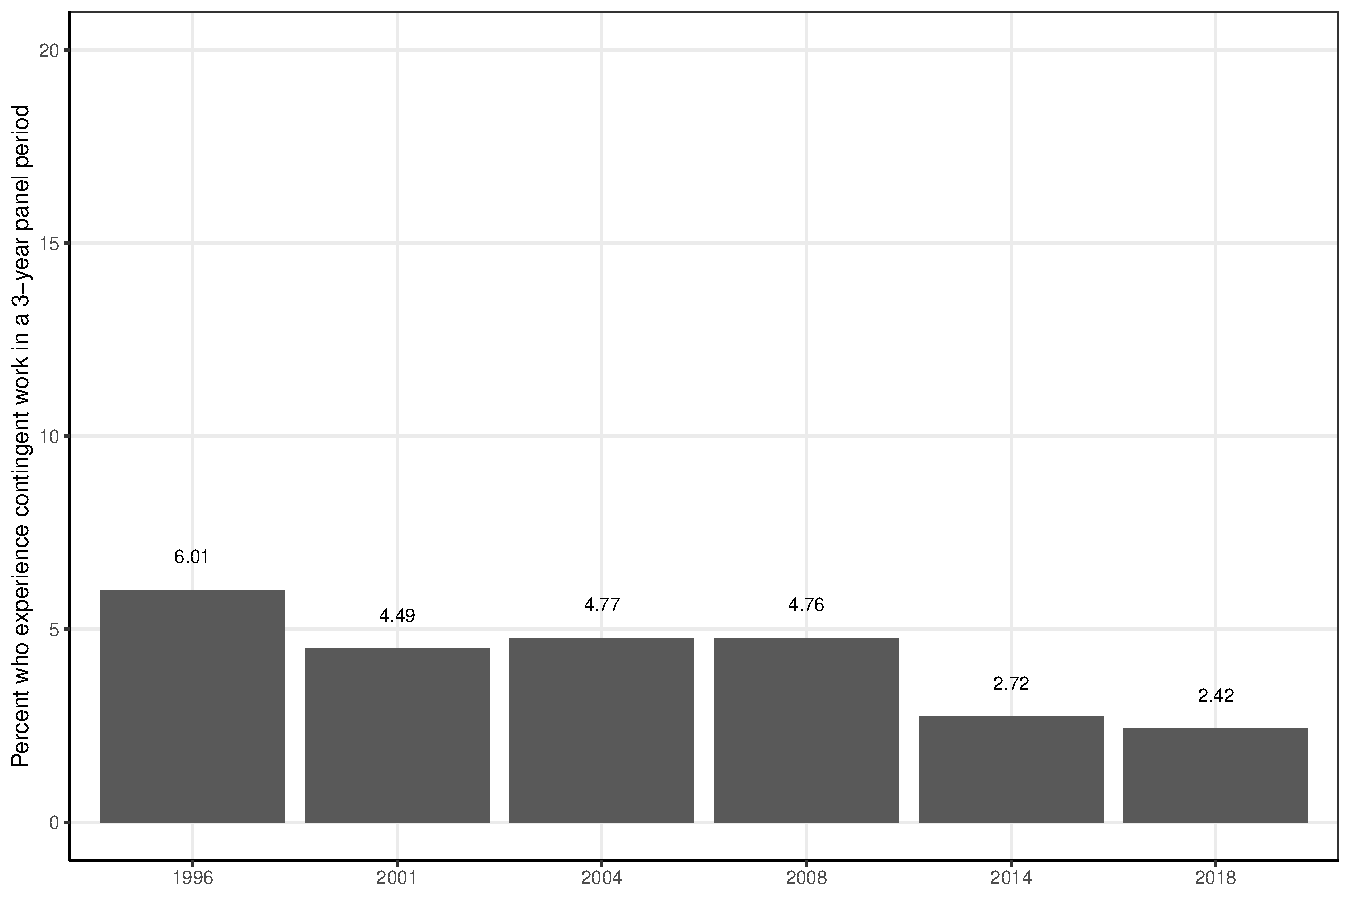
\includegraphics{../graphs/graph_sipp_risk.pdf}}
    \label{graph_sipp_risk}
    \footnotesize{Note: The interpretation of the figure is that, the risk is declining in the percent who experience at least 1 wave (out of 9) of contingent work in a 3 year panel period.  Authors calculations using data from SIPP.}
\end{figure}

\begin{figure}[htp!]
    \caption{Trends in average number of waves with contingent work over time (SIPP)}
    \resizebox{\textwidth}{!}{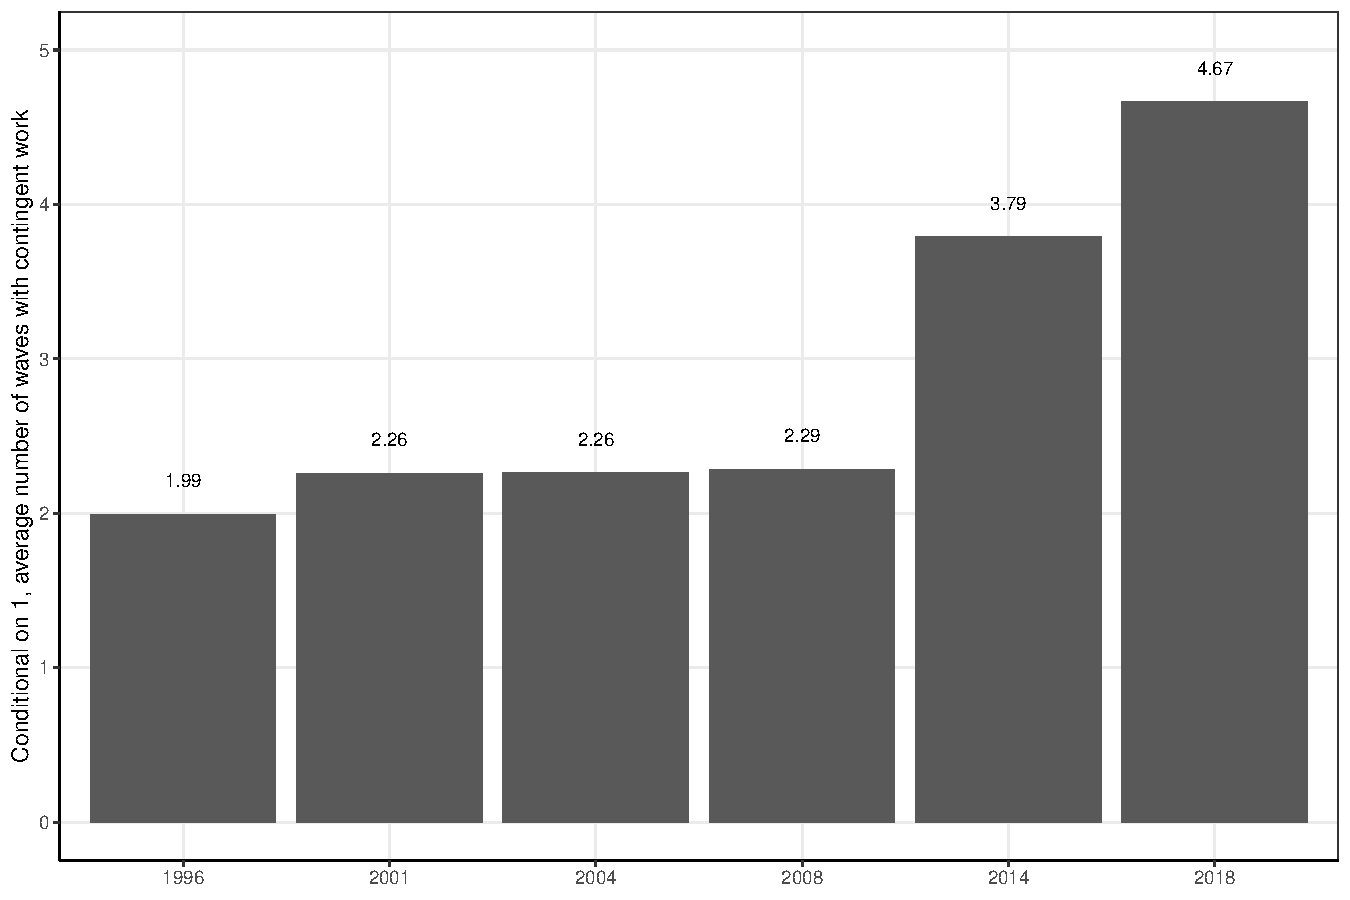
\includegraphics{../graphs/graph_sipp_number_avg.pdf}}
    \label{graph_sipp_number_avg}
    \footnotesize{Note: The interpretation of the figure is that, conditional on at least 1 wave with contingent work, the average number of waves (out of 9) with a contingent work contract is rising.  Authors calculations using data from SIPP.}
\end{figure}

%%%%%%%%%%%%%%%%%%%%%%%%%%%%%%%%
% BIBLIOGRAPHY
%%%%%%%%%%%%%%%%%%%%%%%%%%%%%%%%

\clearpage
\singlespacing
\bibliographystyle{apalike2}
\bibliography{references}

\end{document}
